%=========================================
% 	  Implementierung     		 =
%=========================================

\chapter{Implementierung}

In diesem Kapitel wird das Datenbank-Schema gezeigt und erkl"art, sowie der Quellcode der SQL-Anweisungen.

\section{Datenbank-Schema}
Es gibt in der Datenbank zwei Tabellen und zwei Sichten. Diese sind in ihren entsprechenden Dimensionen unterteilt. Die Tabellen embeddings\underline{  }100 und embeddings\underline{ }50 werden f"ur die SQL-Anweisung ben"otigt, die die Euklidische Distanz berechnet. Die Sichten Liste\underline{ }L"ange\underline{ }100 und Liste\underline{ }L"ange\underline{ }50 werden ben"otigt um f"ur die SQL-Anweisung der Kosinus-"Ahnlichkeit die Formel zu vereinfachen, da man f"ur die Kosinus-"Ahnlichkeit die L"ange braucht.
Zur schnelleren Ermittlung und zur Eindeutigkeit, der Daten, da es keinen Prim"arschl"ussel gibt, wurde noch ein Index auf die Spalten Wort, Jahr, Dimension und Vektor angelegt.\\

\begin{figure}[bth] 
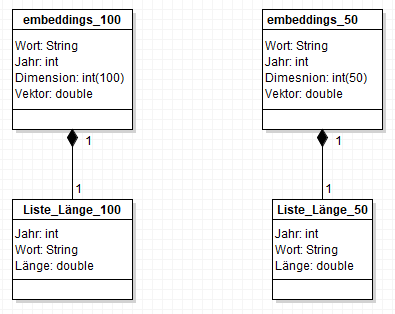
\includegraphics[width=13cm]{Graphics/Datenbank.png}
\caption[Datenbank-Schema]{Struktur der Datenbank}
\end{figure}
\pagebreak

\section{Quellcode}

\subsection{Euklidische Disntanz}
\begin{lstlisting}[style=Java]
    public String selectEuklidisch(String wort1, int jahr1, int jahr2) throws SQLException {
        Statement statement = connection.createStatement();
        String wort = null;
        String sim = null;
        int i = 0;
        StringBuilder stringBuilder = new StringBuilder();
        
        ResultSet rs = statement.executeQuery("SELECT e2.Wort, sqrt(sum(pow(e1.Vektor - e2.Vektor,2))) as sim" +
                " FROM " + TABLE + " e1, " + TABLE + " e2" +
                " WHERE e1.Wort='" + wort1 + "' AND e1.Jahr=" + jahr1 + " AND e2.Jahr=" + jahr2 +
                " AND e1.Dimension=e2.Dimension AND" +
                " (e2.Wort LIKE 'a%' OR e2.Wort LIKE 'b%' OR e2.Wort LIKE 'c%' OR e2.Wort LIKE 'd%' OR e2.Wort LIKE 'e%' OR e2.Wort LIKE 'f%'" +
                " OR e2.Wort LIKE 'g%' OR e2.Wort LIKE 'h%' OR e2.Wort LIKE 'i%' OR e2.Wort LIKE 'j%' OR e2.Wort LIKE 'k%' OR e2.Wort LIKE 'l%'" +
                " OR e2.Wort LIKE 'm%' OR e2.Wort LIKE 'n%' OR e2.Wort LIKE 'o%' OR e2.Wort LIKE 'p%' OR e2.Wort LIKE 'q%' OR e2.Wort LIKE 'r%'" +
                " OR e2.Wort LIKE 's%' OR e2.Wort LIKE 't%' OR e2.Wort LIKE 'u%' OR e2.Wort LIKE 'v%' OR e2.Wort LIKE 'w%' OR e2.Wort LIKE 'x%'" +
                " OR e2.Wort LIKE 'y%' OR e2.Wort LIKE 'z%')" +
                " GROUP BY e2.Wort ORDER BY sim ASC LIMIT 1000");
        while (!rs.isLast()) {
            if (rs.next()) {
                i++;
                wort = rs.getString(1);
                sim = rs.getString(2);
                stringBuilder.append(i + ". " + wort + ", ").append(sim).append("\n");
            }
        }

        return stringBuilder.toString();
    }
\end{lstlisting}
Dieser Code sucht, mit Hilfe des SQL-Kommandos und der Formel zur Berechnung der Euklidischen Distanz, W"orter die nah bei dem gesuchten Wort, hier \textit{'wort1'}, existieren. 



\subsection{Kosinus-"Ahnlichkeit}
\begin{lstlisting}[style=Java]
    public String selectCosinus(String wort1, int jahr1, int jahr2) throws SQLException {
        Statement statement = connection.createStatement();
        StringBuilder stringBuilder = new StringBuilder();
        String wort = null;
        String cos = null;
        int i = 0;

        ResultSet rs = statement.executeQuery("SELECT e2.Wort, sum(e1.Vektor * e2.Vektor) / (l1.Laenge * l2.Laenge) as cos" +
                " FROM " + TABLE + " e1 , " + TABLE + " e2 , " + VIEW + " l1 , " + VIEW + " l2" +
                " WHERE e1.Wort='" + wort1 + "' AND e1.Jahr=" + jahr1 + " AND e2.Jahr=" + jahr2 +
                " AND e1.Dimension=e2.Dimension AND e1.jahr=l1.jahr AND e2.jahr=l2.jahr AND l1.Wort=e1.Wort AND l2.Wort=e2.Wort" +
                " AND (e2.Wort LIKE 'a%' OR e2.Wort LIKE 'b%' OR e2.Wort LIKE 'c%' OR e2.Wort LIKE 'd%' OR e2.Wort LIKE 'e%' OR e2.Wort LIKE 'f%'" +
                " OR e2.Wort LIKE 'g%' OR e2.Wort LIKE 'h%' OR e2.Wort LIKE 'i%' OR e2.Wort LIKE 'j%' OR e2.Wort LIKE 'k%' OR e2.Wort LIKE 'l%'" +
                " OR e2.Wort LIKE 'm%' OR e2.Wort LIKE 'n%' OR e2.Wort LIKE 'o%' OR e2.Wort LIKE 'p%' OR e2.Wort LIKE 'q%' OR e2.Wort LIKE 'r%'" +
                " OR e2.Wort LIKE 's%' OR e2.Wort LIKE 't%' OR e2.Wort LIKE 'u%' OR e2.Wort LIKE 'v%' OR e2.Wort LIKE 'w%' OR e2.Wort LIKE 'x%'" +
                " OR e2.Wort LIKE 'y%' OR e2.Wort LIKE 'z%')" +
                " GROUP BY e2.Wort" +
                " ORDER BY cos DESC" +
                " LIMIT 1000 ");

        while (!rs.isLast()) {
            if (rs.next()) {
                i++;
                wort = rs.getString(1);
                cos = rs.getString(2);
                stringBuilder.append(i + ". " + wort + ", ").append(cos).append("\n");
            }
        }
        return stringBuilder.toString();
    }
\end{lstlisting}
Dieser Code sucht, mit Hilfe des SQL-Kommandos und der Formel zur Berechnung der Kosinus-"Ahnlichkeit, W"orter die nah bei dem gesuchten Wort, hier \textit{'wort1'}, existieren. Dazu wird zur Vereinfachung der Formel die Sichten verwendet.


\subsection{Sichten erstellen}
\begin{lstlisting}[style=Java]
public void createView() throws SQLException {
        Statement statement = connection.createStatement();
        statement.executeUpdate("CREATE VIEW Liste_Laenge_50 ( Jahr, Wort, Laenge ) AS SELECT Jahr, Wort, sqrt(sum(Vektor * Vektor)) as Laenge" +
                " FROM embeddings_50"+
                " GROUP BY Jahr, Wort");
        statement.executeUpdate("CREATE VIEW Liste_Laenge_100 ( Jahr, Wort, Laenge ) AS SELECT Jahr, Wort, sqrt(sum(Vektor * Vektor)) as Laenge" +
                " FROM embeddings_100"+
                " GROUP BY Jahr, Wort");
    }
\end{lstlisting}
Dieser Code erstellt, mit Hilfe des SQL-Kommandos, die Sichten um die L"ange jedes Wortes zu bekommen.

%Hier wird die Implementierung gezeigt und erklärt